\documentclass[../monografia.tex]{subfiles}
\graphicspath{ {images/}{../images/} } 

\begin{document}
% Detalhar neste item os procedimentos realizados para os testes de funcionamento dos sub-sistemas, da inter-relação dos subsistemas e do sistema completo.
% \section{Verificação dos requisitos}

% \section{Testes Realizados} %? Resultados dos Testes

\section{Validação dos Subsistemas} %? Testes Individuais
%Testes de funcionamento dos sub-sistemas

Para os sensores e o display, ao desenvolver cada uma das bibliotecas citadas na seção \ref{firmware}, também desenvolvemos exemplos para a validação de cada um individualmente. 

Utilizando a biblioteca de logging do ESP-IDF \cite{log-esp}, no modo Info, pudemos analisar os dados coletados pelos sensores, assim como os cálculos realizados, através do \textbf{IDF monitor}, uma ferramenta do ESP-IDF que funciona como um terminal serial, comunicando-se com o ESP32. 

Para calcular a \textbf{intensidade} total da luz no ambiente fizemos alguns testes de calibração no LME, com o auxílio do técnico Carlos Ramos. Utilizando uma célula solar padrão com resposta conhecida, pudemos medir a intensidade real de uma luz branca incidindo sobre ela. Colocando em seguida o sensor AS7262, na mesma posição da célula, e incidindo a mesma luz cuja intensidade é agora conhecida, pudemos realizar medições mais precisas. 

Com leituras para diferentes intensidades, somamos os dados lidos pelo sensor para cada espectro, uma vez que o sensor tem como resposta 6 valores proporcionais à energia por unidade de área da luz incidente em cada um de seus filtros internos. 
Dividimos esse valor pelo tempo de integração configurado, cujo funcionamento foi explicado na seção \ref{as7262}, obtendo assim um valor proporcional à intensidade da luz. 	

Com esses dados, mostrados na tabela \ref{table:tabela-luz}, foi possível encontrar uma constante calibrada $\alpha$  para a conversão da leitura. \newpage

%!! tabelas do teste de luz
\begin{table}[h]
\centering
\begin{tabular}{ |c|c|c|c|c|c|c| }
	\hline
	\multicolumn{2}{|c|}{} & \multicolumn{5}{|c|}{\textbf{Intensidade da Luz} ($\mu W/cm^2$)} \\
	\hline
	\textbf{Tempo de Integração} & \textbf{Espectro} & 11000	& 5000 & 20000 & 25000 & 30000 \\
	\hline
	\hline
	\multirow{7}{3em}{84ms (0x1E)} & Violet & 6003&8167&10877&13143 & 16216 \\
	& Blue	&2451	&3368	&4512	&5484	&6822 \\
	& Green	&11271	&15485	&20939	&25654	&30721 \\
	& Yellow &13911	&19084	&25809	&30721	&30721 \\
	& Orange &3404	&4698	&6732	&7801	&9853 \\
	& Red	&1932	&2618	&3608	&4279	&5333 \\
	\hline
	& Soma	&38972	&53420	&72477	&87082	&99666 \\
	\hline
	\multirow{7}{3em}{168ms (0x3C)} & Violet & 12033&	16211&	21585&	26485&	32478\\
	&Blue	&4896	&6577	&8868	&11031	&13647 \\
	&Green	&22588	&30874	&41505	&52153	&61441 \\
	&Yellow	&27844	&38091	&51252	&61441	&61441 \\
	&Orange	&6662	&9184	&12357	&15725	&19672 \\
	&Red	&3790	&5146	&6813	&8689	&10637 \\
	\hline
	&Soma	&77813	&106083	&142380	&175524	&199316 \\
	\hline
\end{tabular}
\caption{Tabela de dados coletados na calibração do sensor AS7262}
\label{table:tabela-luz}
\end{table}
\hfill \break

Encontramos a relação entre a soma lida pelo sensor e a intensidade da luz incidente como a constante $\alpha = \frac{Soma}{\Delta t * I} \approx 41,67$. Assim, podemos calcular os valores da intensidade lida no ambinete $I[\mu W/cm^2]=\frac{Soma}{\Delta t * \alpha}$. Como 1 lux equivale a $1,46*10^-7 W/cm^2$, temos: 

\[I[lux]= 0,146*\frac{Soma}{\Delta t * \alpha}\] \newpage

\section{Validação do Dispositivo} %? Teste Completo

% \subsubsection{Montagem Final}

Foi fabricado um case mecânico em PLA utilizando uma impressora 3D e feita a montagem de um primeiro protótipo, como mostrado na figura \ref{fig:montagem-final}, realizando os ajustes necessários no projeto para o encaixe de todas as peças. 

\begin{figure}[h]
	\centering
	\begin{subfigure}{0.5\textwidth}
		\centering
		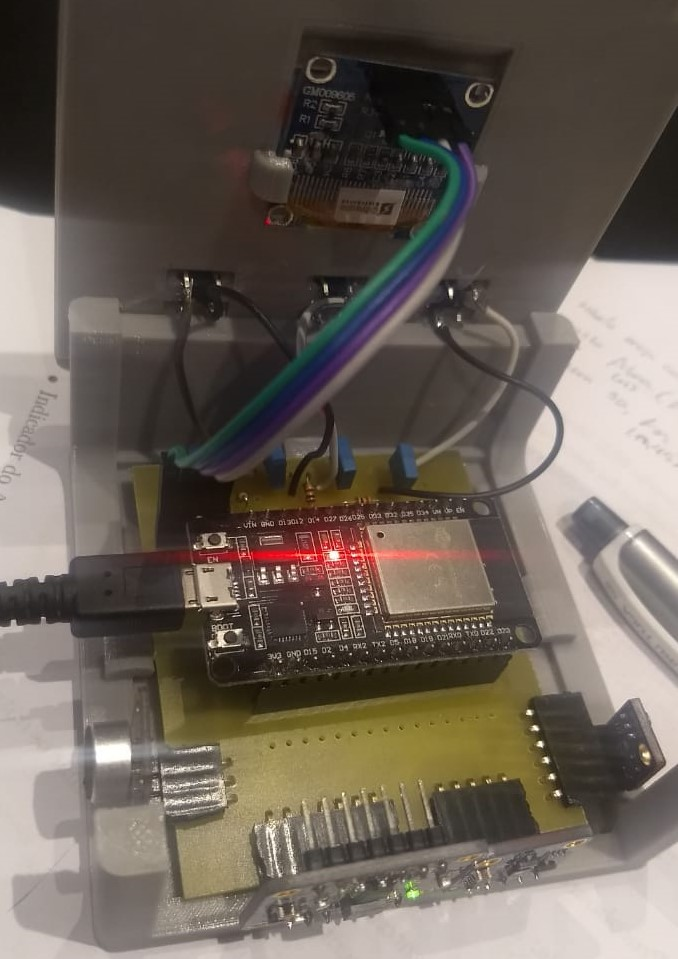
\includegraphics[width=0.8\textwidth]{placa-final}
		\caption{Interna}
		\label{fig:interna}
	\end{subfigure}%
	\begin{subfigure}{0.5\textwidth}
		\centering
		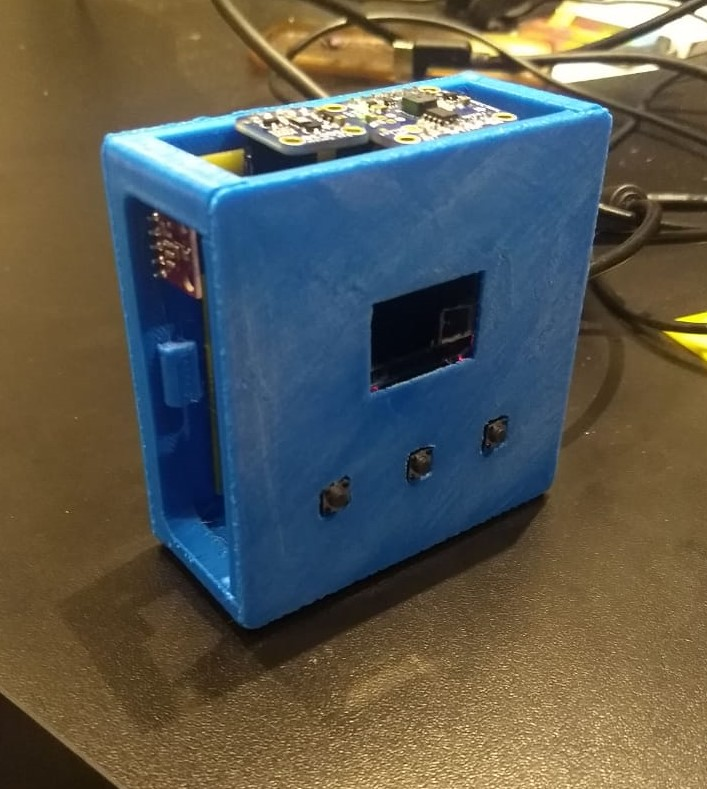
\includegraphics[width=\textwidth]{montagem-final.jpg}
		\caption{Externa}
		\label{fig:externa}
	\end{subfigure}
	\caption{Montagem final do dispositivo}
	\label{fig:montagem-final}
\end{figure}

Para validação de cada subcircuito presente na PCB, utilizamos os mesmos exemplos citados para validação dos sensores e do display, até então testados usando uma protoboard de testes. 

Com o firmware completo desenvolvido, fizemos testes com esse dispositivo, utilizando a mesma biblioteca de Log e o IDF monitor para visualizar as leituras. Os dados dos quatro sensores operando em paralelo podem ser vistos na figura \ref{fig:monitor-sensors}.

%! monitor com dados sensores
\begin{figure}[h]
	\centering
	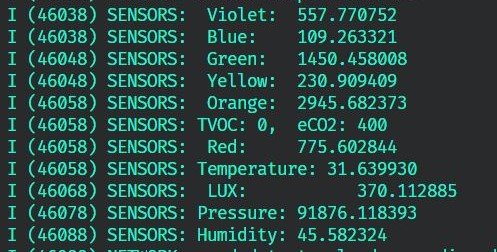
\includegraphics[width=0.6\textwidth]{monitor-sensors}
	\caption{Coleta dos sensores no IDF-Monitor}
	\label{fig:monitor-sensors}
\end{figure}

Cada sensor tem sua coleta sendo feita em uma task individual, isto é, a leitura e os cálculos de um sensor é feito em paralelo aos demais. Dessa forma, a ordem das mensagens sendo apresentadas no monitor terminal podem ocorrer em diferentes ordens a cada iteração, e com dados de dois sensores se intercalando, por exemplo. \newpage

Em seguida, incluímos ao código o envio dos dados via Wi-Fi, como citado na seção \ref{dev-Wi-Fi}, com o dispositivo operando como \textit{gateway}. Os dados das coletas, agora salvos no banco de dados, foram apresentados no dashboard como mostra a figura \ref{fig:dashboard-graphs}.

\begin{figure}[h]
	\centering
	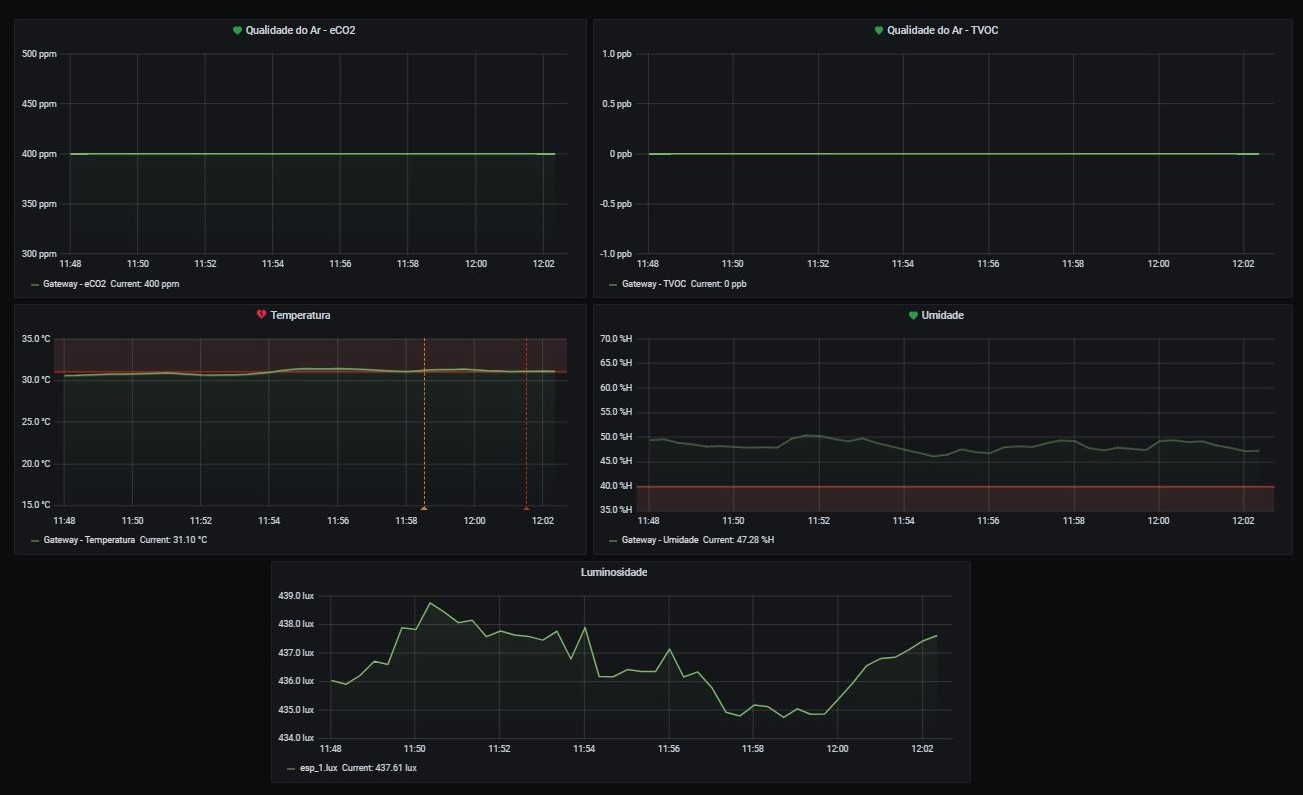
\includegraphics[width=\textwidth]{dashboard-graphs}
	\caption{Gráficos de coletas do Gateway no Dashboard}
	\label{fig:dashboard-graphs}
\end{figure}

Fabricamos outros dois dispositivos para criar a rede BLE-Mesh completa, inicialmente com um dos três dispositivos atuando como "\textit{gateway}". A validação funcional de cada um deles seguiu o mesmo teste do primeiro, coletando dados do ambiente com os sensores e enviando para a plataforma via Wi-Fi. 

Com os nós da rede validados, realizando a coleta e o envio das medições do ambiente, foram feitos os testes dos mesmos nós agora utilizando a arquitetura final proposta, com Bluetooth Mesh. 

Para provisionar os dispositivos na rede Mesh, utilizamos o aplicativo nRF Mesh \cite{nrf-app}, da Nordic Semiconductor. As etapas, comuns aos três dispositivos, estão mostradas na figura \ref{fig:app-nrf-mesh}.

\begin{figure}[h]
	\centering
	\begin{subfigure}[b]{0.22\textwidth}
		\centering
		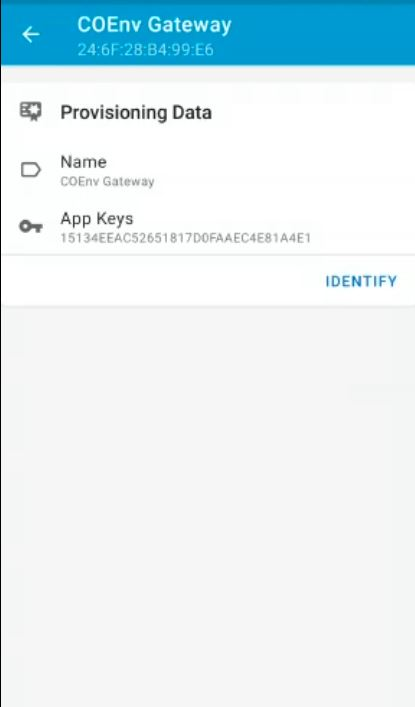
\includegraphics[width=\textwidth]{mesh-bind-1}
		\caption{Identify}
		\label{fig:mesh-bind-1}
	\end{subfigure}
	\begin{subfigure}[b]{0.22\textwidth}
		\centering
		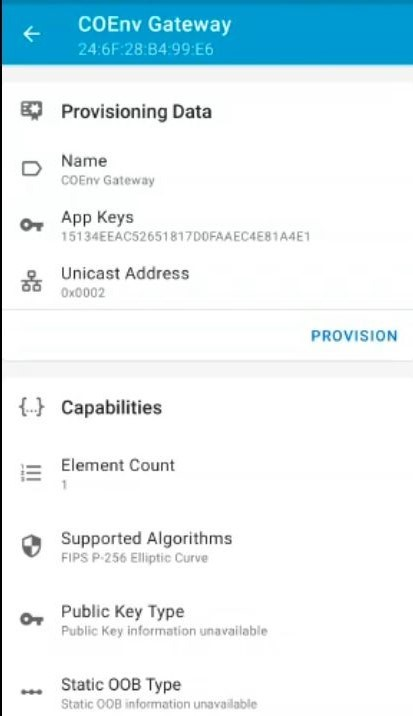
\includegraphics[width=\textwidth]{mesh-bind-2}
		\caption{Provision}
		\label{fig:mesh-bind-2}
	\end{subfigure} %\\*
	\begin{subfigure}[b]{0.22\textwidth}
		\centering
		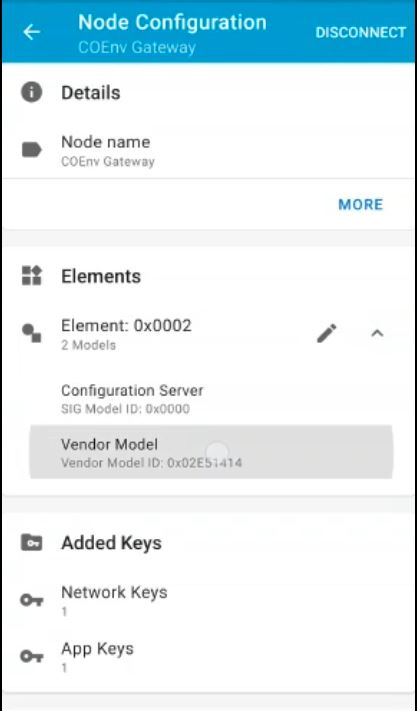
\includegraphics[width=\textwidth]{mesh-bind-3}
		% \caption{$y=2/x$}
		\label{fig:mesh-bind-3}
	\end{subfigure}
	\begin{subfigure}[b]{0.22\textwidth} 
		\centering
		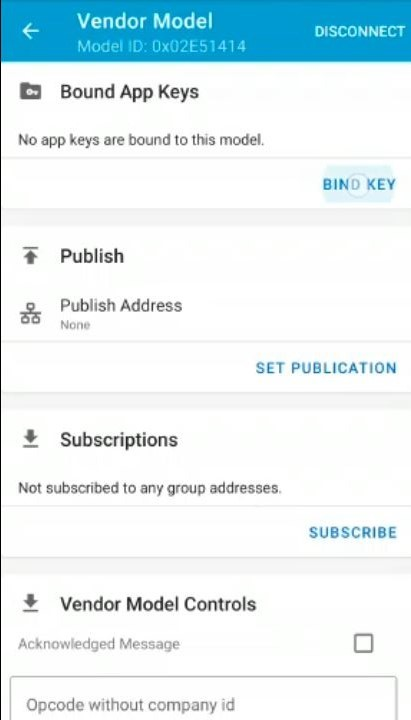
\includegraphics[width=\textwidth]{mesh-bind-4}
		\caption{Bind key}
		\label{fig:mesh-bind-4}
	\end{subfigure}
	\caption{Telas do aplicativo nRF-Mesh}
	\label{fig:app-nrf-mesh}
\end{figure}

\newpage
Além dessas etapas, o dispositivo que atuar como gateway - nesse caso o dispositivo 1 - precisa também se inscrever (subscribe) em um grupo, esse procedimento é msotrado na figura \ref{mesh-subscribe}. Criamos um grupo com endereço 0xC100 para os testes da rede. 

\begin{figure}[h]
	\centering
	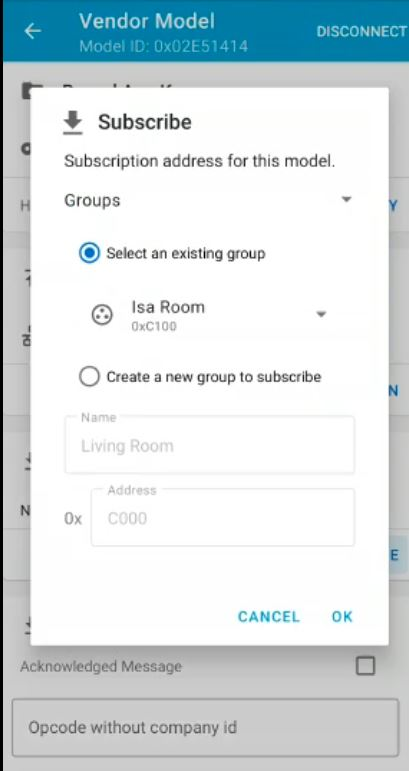
\includegraphics[scale=0.5]{mesh-subscribe.JPG}
	\caption{Tela do app nrf mesh - escolha do grupo}
	\label{mesh-subscribe}
\end{figure}

No dashboard foi possível visualizarmos os dados dos 3 dispositivos em gráficos temporais iguais aos utilizados nos testes funcionais do dispositivo (figura \ref{fig:dashboard-graphs}). Criamos também um segundo dashboard com as últimas leituras dos dispositivos, mostrado na figura \ref{fig:dashboard-medicoes}, de forma a resumir o estado atual da rede de sensores. 

\begin{figure}[h]
	\centering
	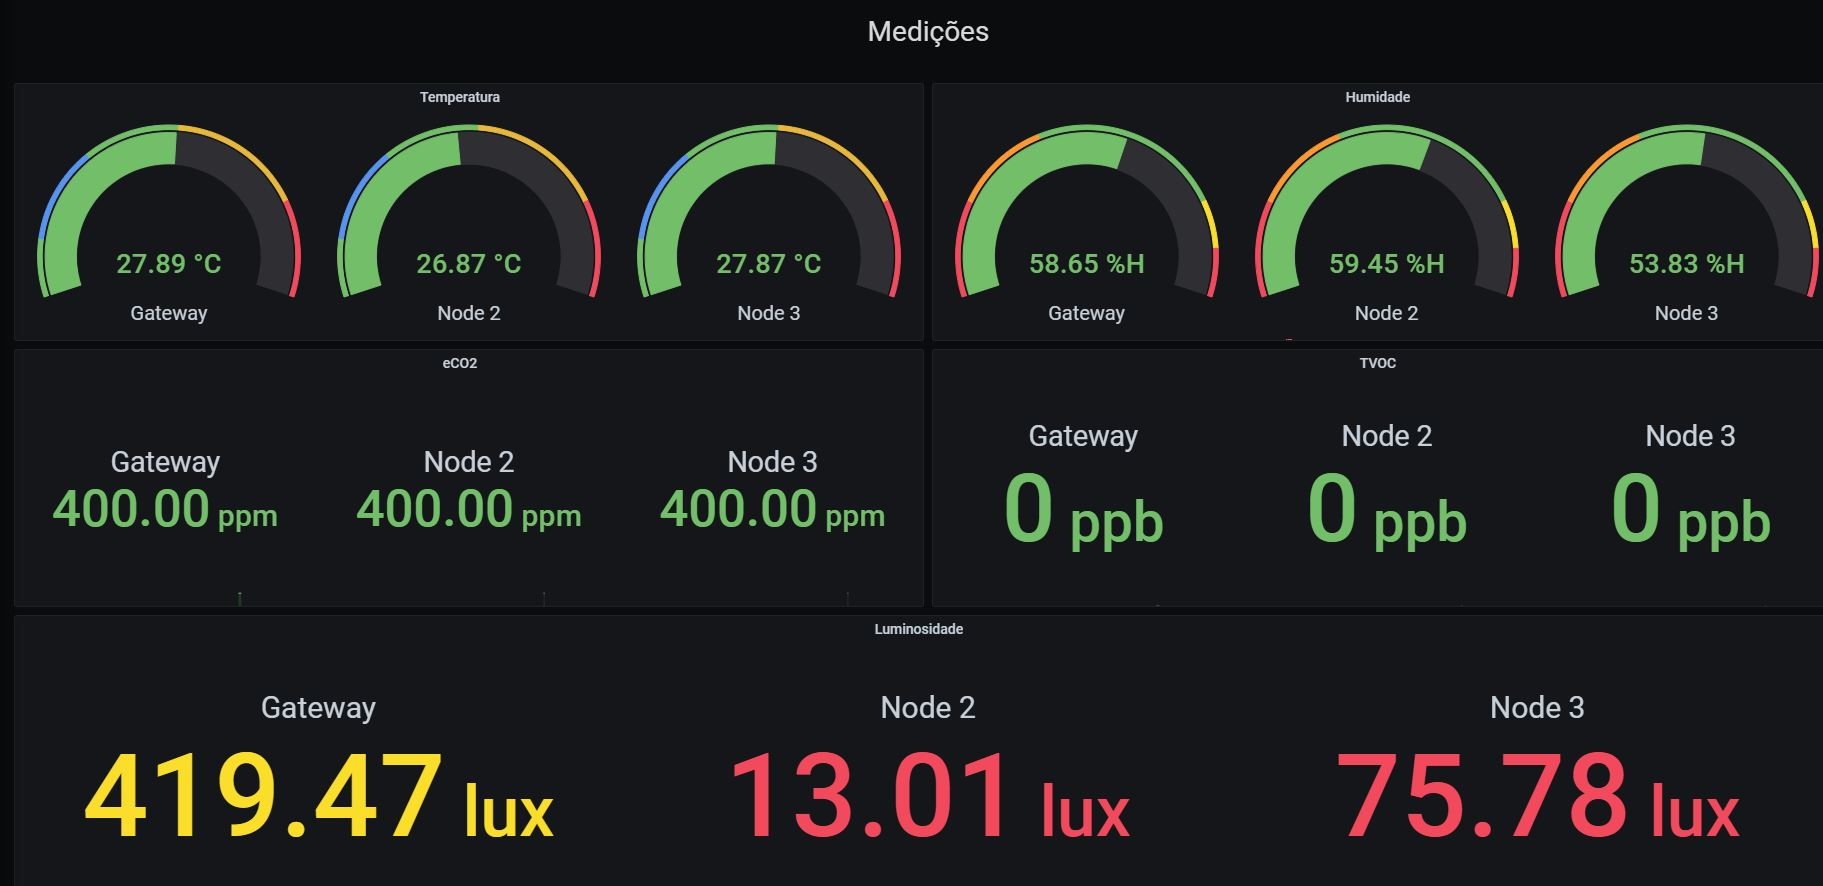
\includegraphics[width=\textwidth]{dashboard-medicoes}
	\caption{Últimas medições dos indicadores no Dashboard}
	\label{fig:dashboard-medicoes}
\end{figure}

\newpage
O dispositivo periodicamente inicia uma coleta de feedback do usuário, junto com uma medição dos indicadores do ambiente. As últimas respostas são apresentadas para o usuário como mostra a figura \ref{fig:dashboard-feedback}. 

\begin{figure}[h]
	\centering
	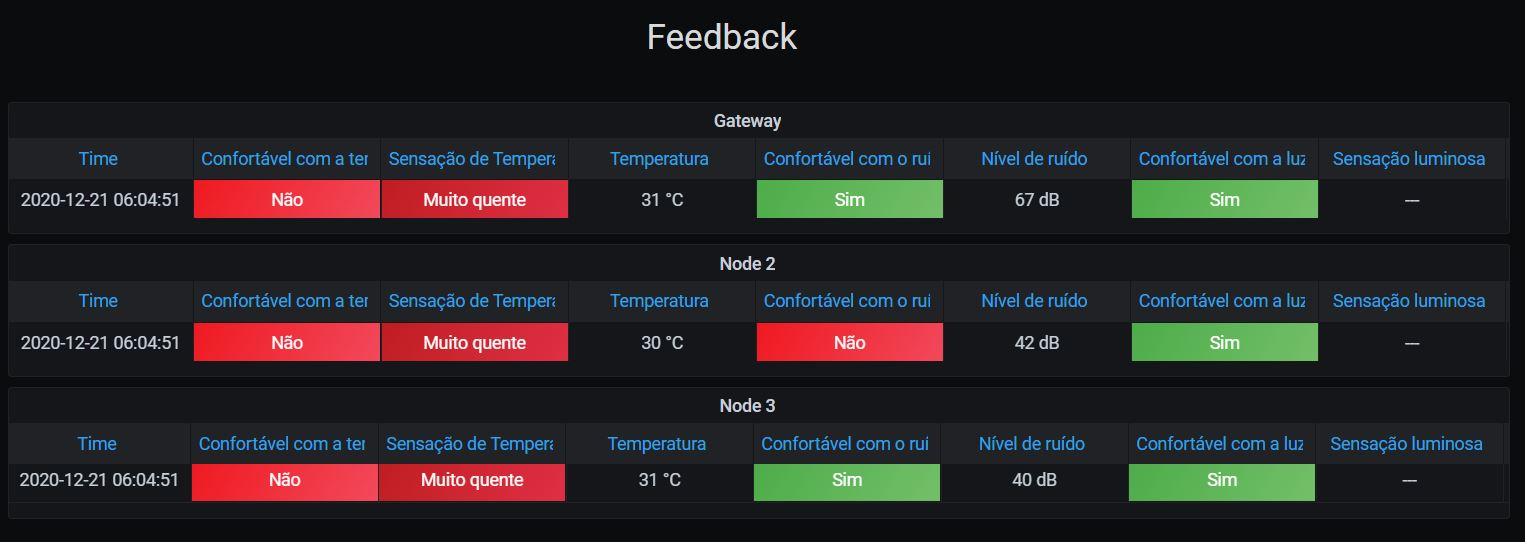
\includegraphics[width=\textwidth]{dashboard-feedback}
	\caption{Feedbacks no Dashboard}
	\label{fig:dashboard-feedback}
\end{figure}

Para cada parâmetro monitorado, foram definidos valores limiares segundo os níves de indicação de qualidade de ambientes para escritórios. A partir desses limiares, foram configurados alertas que são acionados caso o valor médio de certo parâmetro dentro de uma janela de 5 minutos fique acima dos valores definidos e que enviam notificações para um canal no serviço de mensagens \textit{Slack}.    

\begin{figure}[h!]
	\centering
	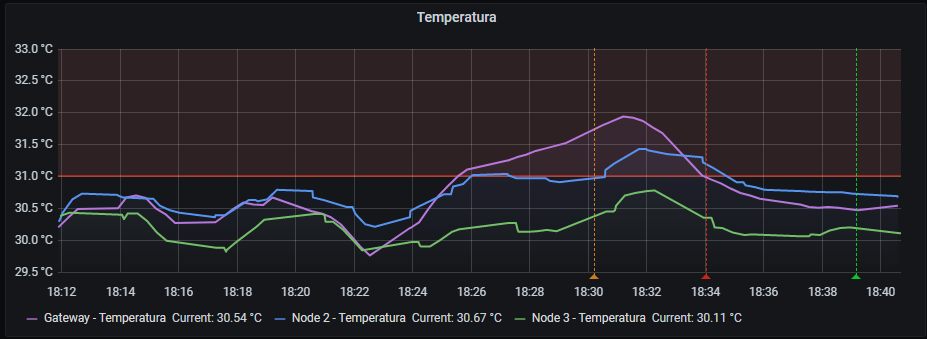
\includegraphics[width=\textwidth]{grafana-temperature-alert.png}
	\caption{Exemplo de ocorrência de alerta de temperatura no Dashboard}
	\label{fig:dashboard-alerta}
\end{figure}

A figura \ref{fig:dashboard-alerta} ilustra um caso em que houve o disparo de uma notificação de alerta: às 18:30, o sistema percebeu que os valores presentes nas séries de cor roxa e azul estavam acima do limiar de 31 °C, que foram monitorados até às 18:34, quando ocorreu o disparo de uma notificação de alerta, ilustrada na figura \ref{fig:slack-alerta}. Finalmente, podemos visualizar que os valores retornaram a níveis abaixo do limiar às 18:39, sendo enviada uma nova notificação para informar essa volta à normalidade, como visto na figura \ref{fig:slack-ok}.


\begin{figure}[h!]
	\centering
	\begin{subfigure}[b]{0.7\textwidth}
		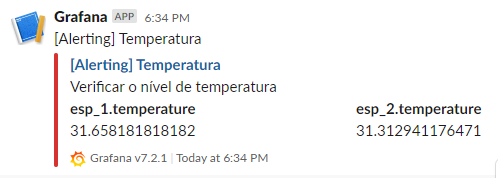
\includegraphics[width=\textwidth]{grafana-slack-alert.png}
		\caption{Notificação de alerta}
		\label{fig:slack-alerta}
	\end{subfigure}
	
	\begin{subfigure}[b]{0.7\textwidth}
		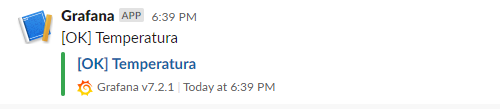
\includegraphics[width=\textwidth]{grafana-slack-ok.png}
		\caption{Notificação de normalidade}
		\label{fig:slack-ok}
	\end{subfigure}

	\caption{Exemplo de recebimento de notificações de alerta no serviço Slack}
	\label{fig:slack-notifications}
\end{figure}



\end{document}